\section{Lecture 4 (27 III 2019)}
\underline{Parity games}:
Eve wins a play $\pi = p_0p_1...$ if $\underset{n \rightarrow \infty}{\lim\sup} (rank(p_n))$ is even,
Adam otherwise.\\
\begin{figure}[H]
	\centering
	\caption{What are $W_E, W_A$ here? (squares are Adam, circles Eve)}
	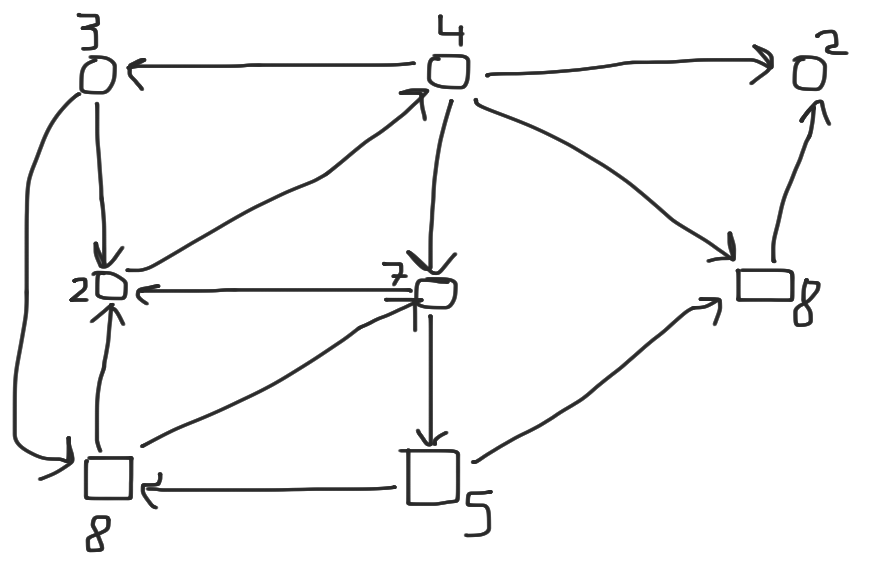
\includegraphics[scale=0.15]{content/graphics/game4}
\end{figure}
\noindent
\underline{General games on labelled graphs}:\\
$Pos_E, Pos_A, Move \in Pos \times Pos$\\
$rank\ :\ Pos \longrightarrow C$\\
Winning criteria:
$W_E \subseteq C^{\omega}, W_A \subseteq C^{\omega}, W_E \cap W_A = \emptyset$\\
\underline{Theorem}: Parity games are positionally determined. We prove for finite
arenas. Some positions are marked $\top$ immediately winning for Eve, $\bot$ immediately winning for Adam.
Induction on \#positions, not marked $\top, \bot$.\\
Induction step: Choose a position $p$ with the highest possible rank $d$, assume (wlog) $d$ is even.
\begin{itemize}
	\item[1] Suppose $p \in Pos_E$. Mark $p$ by $\top$.\\
	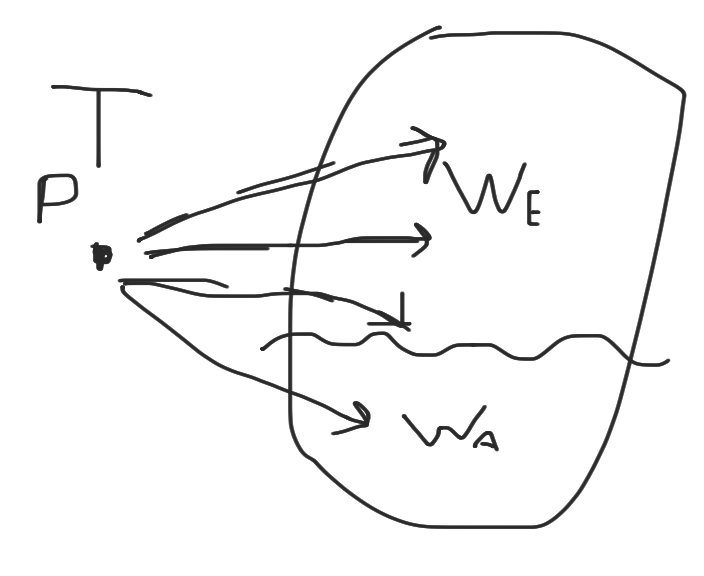
\includegraphics[scale=0.1]{content/graphics/game5}
	\begin{itemize}
		\item[(1a)] There is a move from $p$ to $W_E$.
		\item[(1b)] All moves from $p$ go to $W_A$.
	\end{itemize}
	\item[2] $p \in Pos_A$
	\begin{itemize}
		\item[(2a)] All moves from $p$ go to $W_E$.
		\item[(2b)] There is a move from $p$ to $W_A$.
	\end{itemize}
\end{itemize}

\noindent
Parity game -- $n$ vertices, $d$ ranks. "Simple" algorithm -- $n^{\frac{d}{2} + \Theta(1)}$
